\paragraph{}
Au terme de la compétition, nous étions la seconde entreprise avec le moins de
part de marché mais cela ne nous a pas empêché d'être ceux qui avaient le
cours de l'action en bourse le plus haut. Même aux bénéfices, nous figurions
deuxième. Ceci s'explique facilement par le fait que nous ne vendions que des
téléphones des dernières technologies, avec de nombreuse fonctionnalités.
Étant positionnés sur un marché de luxe, nous étions aptes à pratiquer des
prix élevés nous permettant ainsi de jouir de marges conséquentes. Le bénéfice
dégagé par unité de production était donc particulièrement élevé dans notre
entreprise.

\paragraph{}
Notre choix de commencer à développer assez tôt les techologies 3 et 4 a payé
puisqu'au cours de la 9ème année, nous étions parmi ceux qui avaient les coûts
de production les plus bas
\footnote{Voir figures \ref{coutTech3} et \ref{coutTech4}.}
pour ces deux technologies particulièrement prisées et rentables. Nous avons
ainsi bien profiter de l'effet d'expérience, notre choix de nous passer de la
technologie 2 semble donc avoir porté ses fruits. Il est aussi possible de
remarquer qu'une seule entreprise était réellement capable de rivaliser avec
nous sur les coûts de production de la technologie 4 (ERATEL). En revanche,
elle avait un coût de production bien plus élevé en ce qui concerne la
technologie 3. On peut donc considérer que ce qui nous a réellement permis de
nous démarquer a été notre aptitude a être compétitif de manière simultanée
sur les deux marchés les plus fructueux. De plus, nous avons pu observer qu'en
nous plaçant sur des marchés haut-de-gamme, le problème de gestion des stocks
devenait moins critique.

\begin{figure}
  \caption{\label{coutTech3}Cout de production de la technologie 3}
  \centering
  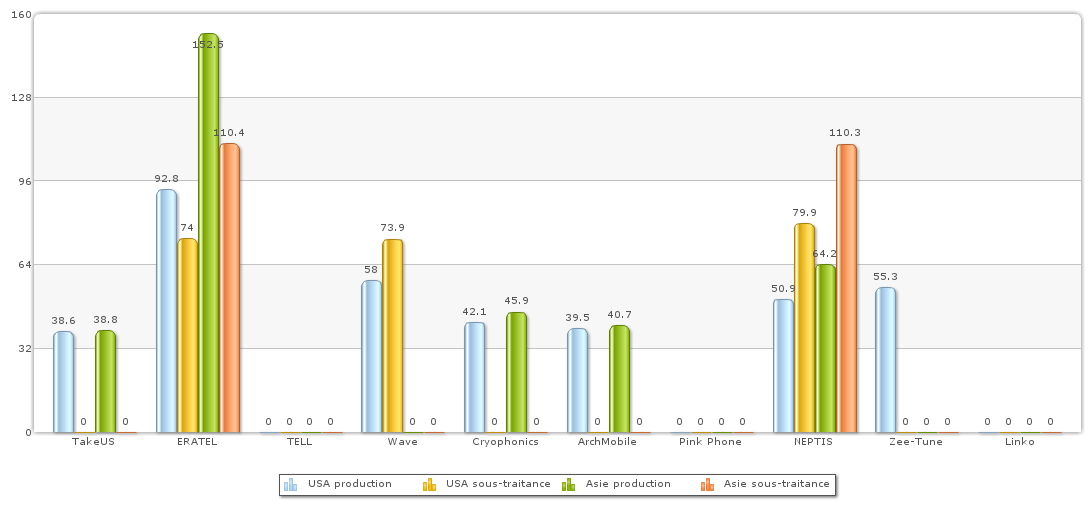
\includegraphics[width=\textwidth]{CoutTech3.png}
\end{figure}

\begin{figure}
  \caption{\label{coutTech4}Cout de production de la technologie 4}
  \centering
  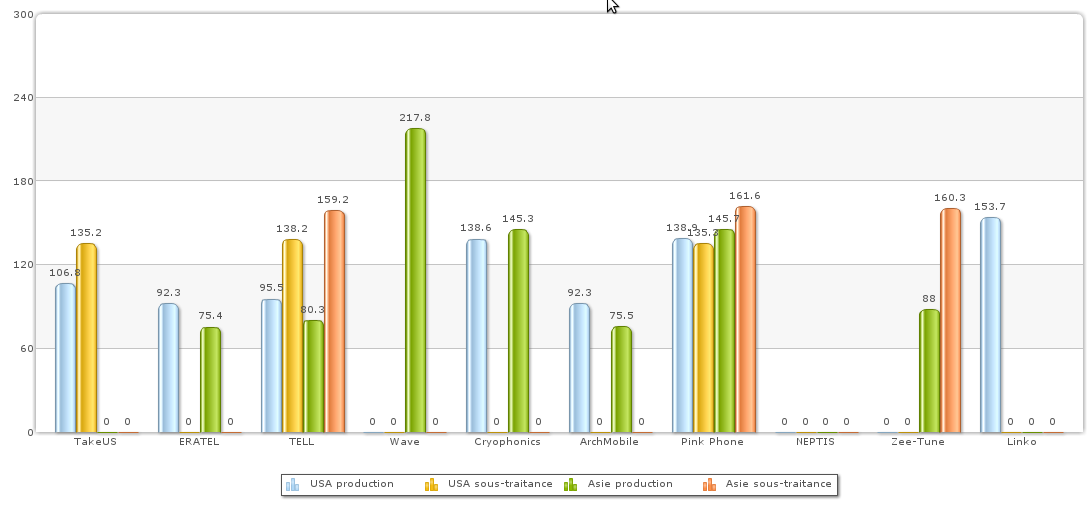
\includegraphics[width=\textwidth]{CoutTech4.png}
\end{figure}
